% Copyright 2017 Rebecca Skinner
%
% This work is licensed under the Creative Commons
% Attribution-ShareAlike 4.0 International License. To view a copy of
% this license, visit http://creativecommons.org/licenses/by-sa/4.0/
% or send a letter to Creative Commons, PO Box 1866, Mountain View, CA
% 94042, USA.
\documentclass{beamer}

\title{Monadic Error Handling in Go}
\subtitle{Breaking Beyond Common Go Idioms}
\author{Rebecca Skinner\\ \small{@cercerilla}}
\institute{Asteris, LLC}
\date{\today}

\mode<presentation> {\usetheme{metropolis}}

\usepackage[english]{babel}
\usepackage{times}
\usepackage[T1]{fontenc}
\usepackage{hyperref}
\usepackage{listings}
\usepackage{listings-golang}
\usepackage{color}
\usepackage{amsmath}
\usepackage{csquotes}
\usepackage{verbatim}
\usepackage{fontspec}
\usepackage{pbox}

\definecolor{comment}{rgb}{145,175,188}
\definecolor{keyword}{rgb}{157,163,199}
\definecolor{string}{rgb}{155,204,174}

\lstset{ % add your own preferences
  basicstyle=\tiny,
  showspaces=false,
  showtabs=false,
  numbers=none,
  numbersep=5pt,
  showstringspaces=false,
  stringstyle=\color[rgb]{0.16, .47, 0},
  tabsize=1
}

\newcommand{\chref}[3] {
  {\color{#1} \href{#2}{\underline{#3}}}
}

\AtBeginSection[]{
  \begin{frame}
    \vfill
    \centering
    \begin{beamercolorbox}[sep=8pt,center,shadow=true,rounded=true]{title}
      \usebeamerfont{title}\insertsectionnumber \\ \insertsectionhead\par%
    \end{beamercolorbox}
    \vfill
  \end{frame}
}

\AtBeginSubsection[]{
  \begin{frame}
    \vfill
    \centering
    \begin{beamercolorbox}[sep=8pt,center,shadow=true,rounded=true]{title}
      \usebeamerfont{title}\insertsectionnumber.\insertsubsectionnumber\\\insertsubsectionhead\par%
    \end{beamercolorbox}
    \vfill
  \end{frame}
}

\begin{document}
\begin{frame}
  \titlepage{}
  \begin{center}
    \small{\chref{blue}{http://creativecommons.org/licenses/by-sa/4.0/}{LICENSE}}
  \end{center}
\end{frame}

\begin{frame}
  \frametitle{External Resources}
  Find links below to the source code of this presentation, as well as
  the full source code for our example application and the gofpher
  library.
  \\\vfill
  \begin{itemize}
  \item sample code: \chref{blue}{https://github.com/rebeccaskinner/agile17-sample}{agile17-sample}
  \item reference library: \chref{blue}{https://github.com/rebeccaskinner/gofpher}{gofpher}
  \item slides: \chref{blue}{https://github.com/rebeccaskinner/presentations/tree/agile-tech-2017/agile_tech_conference_2017}{source code}
  \end{itemize}
\end{frame}

\section{Introduction}
\begin{frame}
  \frametitle{Background}
  Over the last two years that I've been working with Go I've come to
  believe that some of it's idioms are a detriment to quality. In this
  presentation we'll focus on error handling, and how a decidedly
  non-idiomatic approach might make our lives simpler.
\end{frame}

\begin{frame}
  \frametitle{What We'll Cover}
  \begin{itemize}
  \item An overview of Go's philosophy and idioms
    \pause
  \item How idiomatic error handling in go works
    \pause
  \item The problems with error handling in go
    \pause
  \item An introduction to monads and the Gofpher library
    \pause
  \item Using Gofpher in real-world code
    \pause
  \item Idioms and the lessons we've learned
  \end{itemize}
\end{frame}

\section{What Makes Go Go?}
\begin{frame}
  \frametitle{Go's History}
  Go was created at Google by a team including Rob Pike and Ken
  Thompson.  It was designed to help make the development of
  microservices easier, and to address common criticisms of C++ and
  Java.  It's often called ``a better C''.
\end{frame}

\begin{frame}
  \frametitle{Easy}
  Go is a language that strives to be easy.  In most cases the
  language appears to prefer accessbility and immediate producivity,
  especially for developing small network services, over any other
  concern.

  Some key factors that keep go easy:
  \begin{itemize}
  \item Statically compiled language
  \item Rudimentary static type system, with type inference
  \item Garbage Collected
  \item {\tt go get} for libraries and tools
  \item Procedural, with C-Like syntax
  \item {\tt gofmt} and {\tt goimports} to keep code consistent
  \end{itemize}
\end{frame}

\begin{frame}
  \frametitle{Unambigious}
  Go's syntax was designed to be unambigious, and easily parsable by
  both humans and machines.  To this end, Go has focused on syntacic
  constructs that are specific and universal.

  Key decisions:
  \begin{itemize}
    \item Interface-only polymorphism
    \item Static type system
    \item User-defined types limited to Structs and Interfaces
  \end{itemize}
\end{frame}
\begin{frame}
  \frametitle{Obvious}
  Go is designed to be obvious, both to the writer who should not have
  to think about how to use an API, and to a reader who should be able
  to clearly understand what any piece of code is doing with minimal
  understanding of the surrounding context.
\end{frame}
\begin{frame}
  \frametitle{Idiomatic}
  Go is an opinionated language.  While many idioms are not enforced
  by the compiler, may tools exist to ensure that go code conforms to
  designed and community established idioms.
\end{frame}
%%%
\section{Error Handling in Go}
\begin{frame}
  \frametitle{A Visualization of Error Handling}
    \begin{center}
    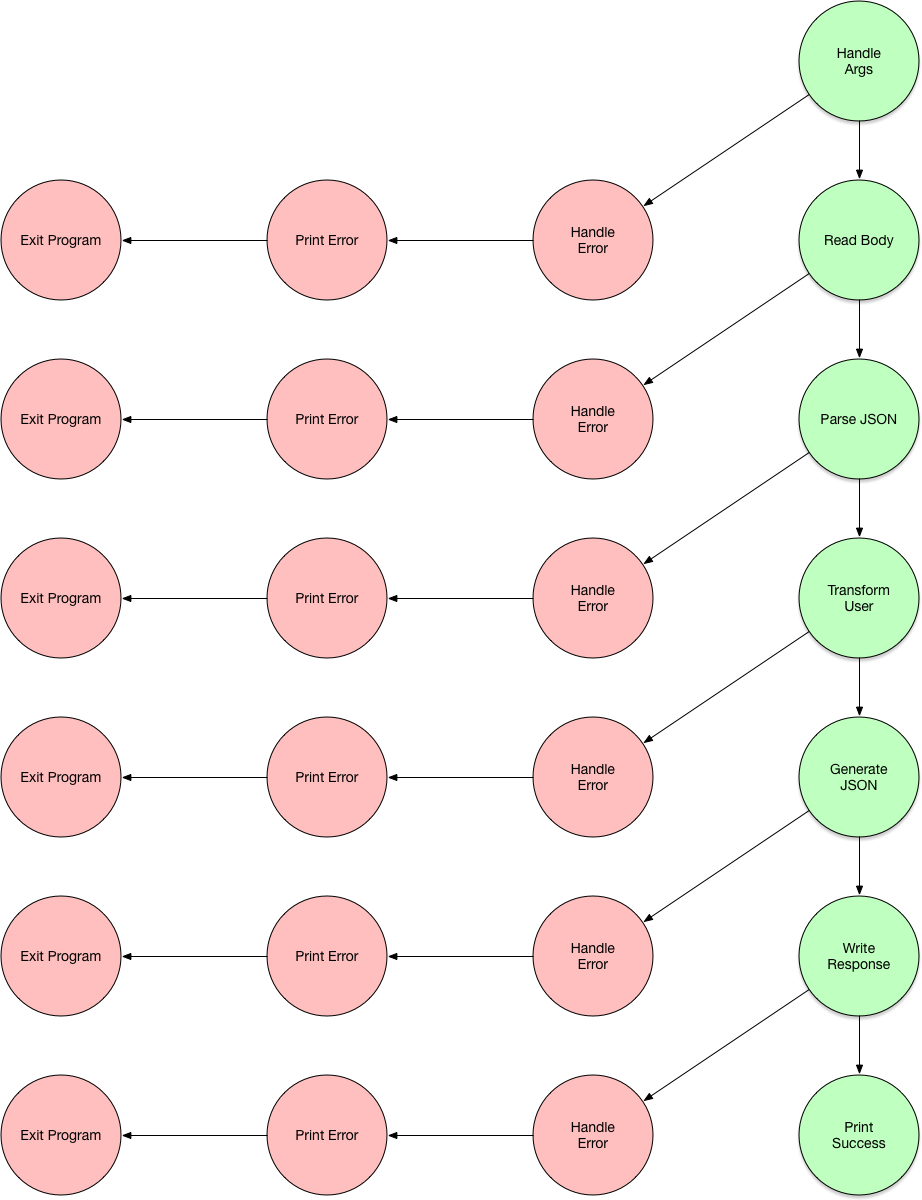
\includegraphics[height=.85\paperheight]{images/curr_err_graph}
  \end{center}
\end{frame}

\subsection{Error Handling by Convention}
\begin{frame}
  \frametitle{How Do We Handle Errors?}
  Idiomatic error handling in go favors a manual and straightfoward
  approach. Each function that can fail returns an error, and each
  error is checked with, or immediately following, the call.  When an
  error occurs it is handled or propegated up the call chain until it
  can be addressed.
\end{frame}

\begin{frame}
  \frametitle{Error is an Interface}
  Errors in go typically implement the {\tt error} interface.  The
  common patterns we see with errors are:

  \begin{itemize}
  \item {\tt nil} indicates the absense of an error
  \item Specific errors are defined as constants, and compared by value
  \item Errors may be nested, to provide context for a failure
  \end{itemize}

  This approach isn't problematic per-se, but as we'll see having
  errors as their own kind of stand-alone value can cause some
  problems.
\end{frame}

\begin{frame}[fragile]
  \frametitle{Multi-Returns}
  Go supports functions that return more than one value.  This is the
  most prominent feature of how go deals with errors. Most functions
  that can fail return a tuple of a value and an error.
  \par\pause
\begin{lstlisting}[language=Golang]
// NewFromJSON returns a new user from the deserialized json, or an error
func NewFromJSON(s []byte) (*User, error) {
        u := &User{}
        err := json.Unmarshal(s, u)
        return u, err
}
\end{lstlisting}
\end{frame}

\begin{frame}[fragile]
  \frametitle{In-Line Checking}
  Go's errors are handled in line, explicitly.  By convention, each
  time a function is called that may return an error, we check the
  error immediately and
  \par\pause
\begin{lstlisting}[language=Golang]
newUserJSON, err := json.Marshal(newUser)
if err != nil {
        fmt.Println("failed to marshal new user: ", err)
        os.Exit(1)
}
\end{lstlisting}
\end{frame}

\begin{frame}[fragile]
  \frametitle{Error Propagation}
  When a function encounters an error in a go application, the
  conventional approach is to return it up the call chain.  Errors may
  be returned unmodified or, as in our example below, wrapped with
  context.
  \par\pause
\begin{lstlisting}[language=Golang]
func NewFromJSON(s []byte) (*User, error) {
        u := &User{}
        if err := json.Unmarshal(s, u); err != nil {
                return nil, errors.Wrap(err, "failed to deserialize JSON data")
        }
        return u, nil
}
\end{lstlisting}
\end{frame}

\subsection{The Problem with the Convention}
\begin{frame}
  \frametitle{Why Error Handling Doesn't Scale}
  Idiomatic approaches to error handling can become problematic when
  we start dealing with larger functions that have many potential
  points of failure.
  \\\vfill
  \begin{itemize}
    \item There is no enforcement mechnanism to ensure we check errors
    \item Errors are often checked several times, with potentially inconsistent handling
    \item Business logic is obscured by verbose error checking
  \end{itemize}
\end{frame}

\begin{frame}
  \frametitle{Error Handling Is Error Prone}
  When we are calling functions with multiple return values, go
  enforces that we capture, or explicitly ignore, each return
  value. Unfortunately, there is no way for the language to ensure
  that we are actually handling the error values.
\end{frame}

\begin{frame}[fragile]
  \frametitle{Write Everything Twice}
  Because it's idiomatic to pass errors up the chain, it's very common
  to find our code handling ever error two or more times.

  In the example below there is a single error condition: the user did
  not supply enough command line arguments. We end up checking for the
  error twice:
  \par\pause
\begin{lstlisting}[language=Golang]
func getArgs() (*config, error) {
        args := os.Args
        if len(args) < 3 {
                return nil, errors.New("insufficient number of arguments")
        }
        return &config{endpoint: args[1], username: args[2]}, nil
}

func main() {
        config, err := getArgs()
        if err != nil {
                fmt.Println(err)
                os.Exit(1)
        }
}
\end{lstlisting}
\end{frame}

\begin{frame}
  \frametitle{Verbosity}
  Function calls in go are frequently accompanied by 3+ lines of error
  handling. This can cause several problems when we want to write
  maintainable code:
  \par\pause
  \begin{itemize}
  \item Business logic is obscured by error handling
    \pause
  \item Refactoring becomes error prone
    \pause
  \item Every additional code path adds more tests
    \pause
  \item We need more mocking ensure we're fully exercising our code paths
  \end{itemize}
\end{frame}

\begin{frame}
  \frametitle{The Density of Error Handing vs. Business Logic}
  \begin{center}
    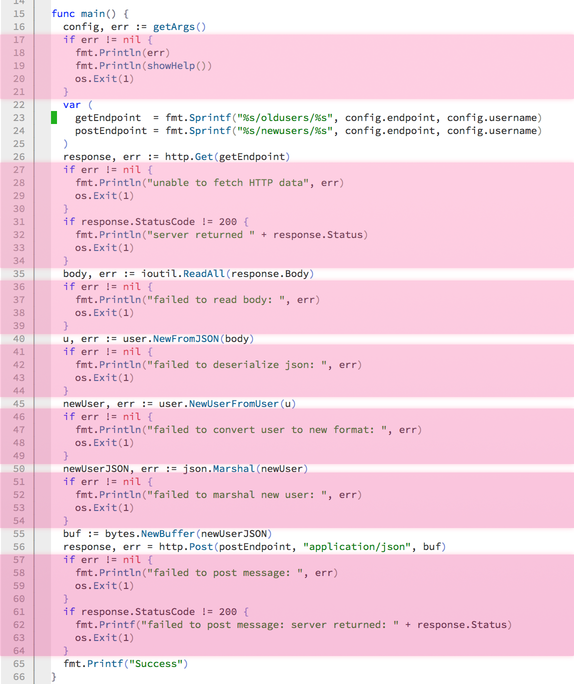
\includegraphics[height=.85\paperheight]{images/current_errors_highlighted}
  \end{center}
\end{frame}

\section{How Can We Do Better?}
\begin{frame}
  \frametitle{Error Handling}
  {\it ``Better Code''} is hard to define in the general case, so let's
  narrow our scope down to error handling and try to define
  {\it better}.
\end{frame}

\begin{frame}
  \frametitle{What if Code Looked Like This}
  \begin{center}
    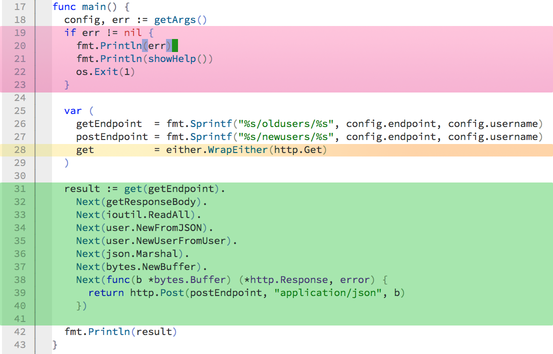
\includegraphics[width=.85\paperwidth]{images/monadic_highlighted}
  \end{center}
\end{frame}

\begin{frame}
  \frametitle{Terseness}
  {\bf Terseness}: Using fewer statements.
  \par\pause
  Terseness is valuable (up to a point) because every statement is a
  potential error.  As we reduce the number of LOC we reduce the
  expected number of bugs in the application.
  \vfill
  \begin{itemize}
  \item Irrespective of projects defect density, more KLOC == more bugs
  \item Code on the screen is a mental cache
  \item Each branch is an opportunity for a mistake
  \end{itemize}
\end{frame}

\begin{frame}
  \frametitle{Expressiveness}
  {\bf Expressiveness}: The amount of meaning in a single statement.
  \par\pause
  The more meaning we pack into a statement, the fewer statements we
  have, giving us more terse code.  Expressive code is also easier to
  read because it allows a user to work at a higher level of
  abstraction and be less bogged down in the details.
  \vfill
  \begin{itemize}
  \item More meaning per statement improves terseness
  \item Higher expressiveness makes code easier to understand
  \end{itemize}
\end{frame}

\begin{frame}
  \frametitle{Robustness}
  {\bf Robustness}: Resiliance against mistakes, errors, and changes to the code.
  \par\pause
  Robustness in our code means that the structure of our code
  automatically guards against errors.  When we have patterns and
  idioms that help us guard against bugs without having to think about
  it, we're less likely to miss things.
  \vfill
  \begin{itemize}
  \item Prohibiting errors makes code safer
  \item Guaranteed safety makes tests simpler
  \end{itemize}
\end{frame}

\section{Monads: A Real Life Approach}
\begin{frame}
  \begin{center}
    
\includegraphics[height=.85\paperheight]{images/burrito}
  \end{center}
\end{frame}

\begin{frame}
  \frametitle{Where Did Monads Come From?}
  The use of monads for handling computational pipelines was initially
  developed in the haskell community.  It has since become popular in
  other ML-family languages like Elm, Typescript, and Idris.

  Languages outside of the ML family, including scala and ATS, also
  have support for monadic computations.

  Borrowing idioms from other languages can provide insights into how
  to improve code in a language we are using.
\end{frame}

\begin{frame}
  \frametitle{What Are Monads?}
  A monad is a kind of very general interface that arises very
  naturally from a lot of code.  At their heart, monads give us a way
  of keeping track of context as a side effect of operating on some
  data.

  \par\pause
  An implementation of {\tt Monad} needs to be able to hold some
  data. In addition it needs to be able to support just two functions:
  \begin{itemize}
  \item {\tt Return} Creates a new container with a value in it.
  \item {\tt Bind} Takes a value in a container, and a function that
    returns a value in a container, calls the function with the value,
    and joins the two containers.
  \end{itemize}
\end{frame}

\begin{frame}
  \begin{center}
    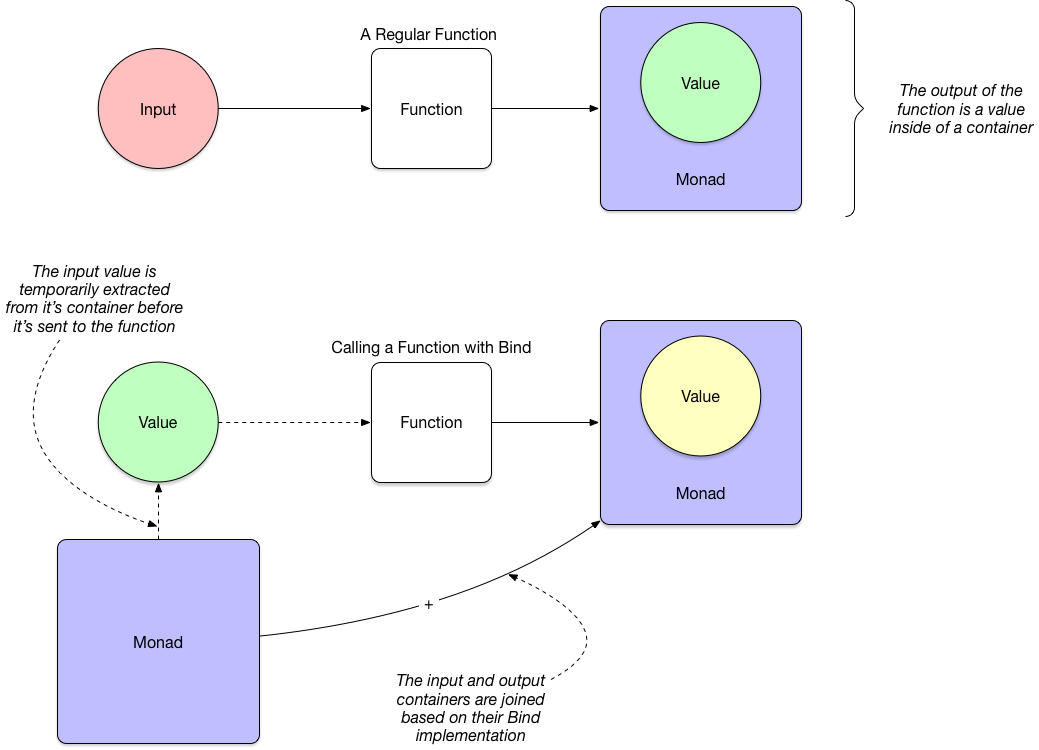
\includegraphics[height=.85\paperheight]{images/monads_visualized}
  \end{center}
\end{frame}

\subsection{How Can Monads Help Us Write Better Code?}
\begin{frame}
  \frametitle{Errors are Context}
  The question of whether or not an error occured is part of the
  context of a value.  In other words, when a function can fail, it's
  result is \emph{Either} and error occured, or we have an output
  value.
\end{frame}

\begin{frame}[fragile]
  \frametitle{The Either Monad}
\begin{lstlisting}[language=Golang]
package either

type Either struct {
        Value interface{}
        Err   error
}

func Return(i interface{}) Either {
        return Either{Value: i}
}

func (e Either) Bind(f func(i interface{}) Either) Either {
        if e.Err != nil {
                return e
        }
        return f(e.Value)
}
\end{lstlisting}
\end{frame}

\begin{frame}[fragile]
  \frametitle{A Contrived Example}
  Here's a contrived example of using {\tt EitherM} to catch errors in a pipeline.
\begin{lstlisting}[language=Golang]
func increment(i int) (int, error) {
    if i >= 10 {return i, fmt.Errorf("can't increment: %d is >= 10", i)}
    return i + 1, nil
}
func double(i int) (int, error) {
    if i%2 == 0 {return i, fmt.Errorf("can't double: %d is even", i)}
    return i + i, nil
}
func main() {
    succ := either.WrapEither(increment)
    dbl := either.WrapEither(double)
    fmt.Println(succ(12).AndThen(dbl))
    fmt.Println(dbl(3).AndThen(succ))
    fmt.Println(dbl(3).AndThen(succ).AndThen(dbl))
    fmt.Println(dbl(3).AndThen(succ).AndThen(succ).AndThen(dbl))
}
\end{lstlisting}
Output:
\begin{lstlisting}
Left (can't increment: 12 is >= 10)
Right (7)
Right (14)
Left (can't double: 8 is even)
\end{lstlisting}
\end{frame}

\begin{frame}
  \frametitle{Monadic Pipelines for Readability and Correctness}
  A \emph{monadic pipeline} is a series of function calls connected in order
  with calls to {\tt Bind}.

  \par\pause
  Monadic pipelining allows us to construct a chain of function calls
  without having to worry about explicitly addressing failures.  Since
  each call to {\tt Bind} returns a new {\tt Either} monad, we can
  focus on our business logic and let the error context be handled
  implicitly.
\end{frame}

\begin{frame}
  \begin{center}
    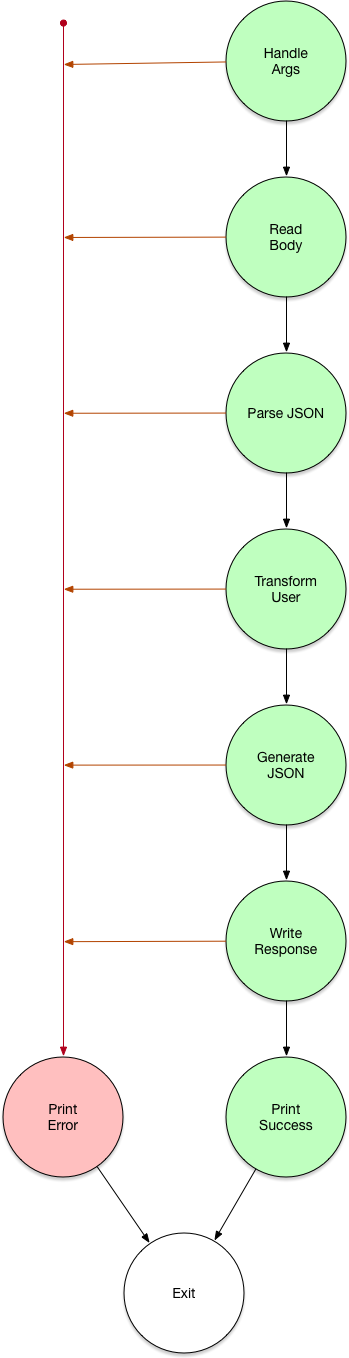
\includegraphics[height=.95\paperheight]{images/rails_graph}
  \end{center}
\end{frame}

\begin{frame}[fragile,t]
  \frametitle{Comparing Traditional and Monadic Code}
  \begin{columns}
    \begin{column}{.45\paperwidth}
      \begin{figure}
        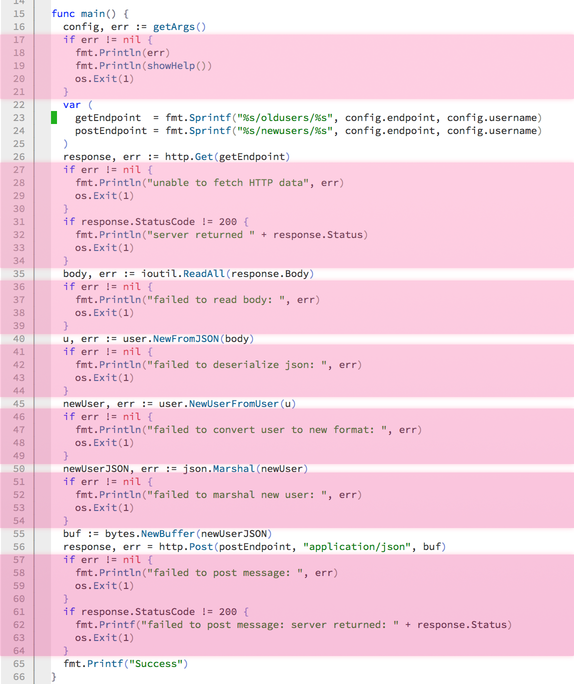
\includegraphics[keepaspectratio,height=\paperheight,width=.4\paperwidth]{images/current_errors_highlighted}
        \caption{Traditional Code}
      \end{figure}
    \end{column}
    \begin{column}{.45\paperwidth}
      \begin{figure}
        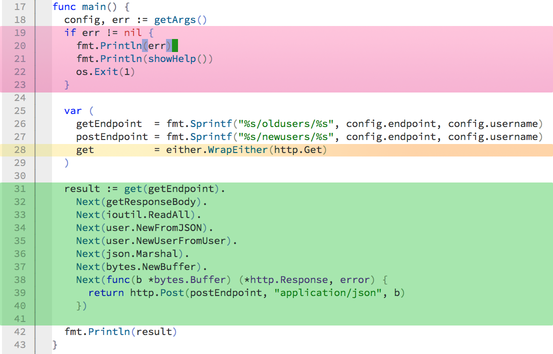
\includegraphics[keepaspectratio,height=\paperheight,width=.4\paperwidth]{images/monadic_highlighted}
        \caption{Monadic Code}
      \end{figure}
    \end{column}
  \end{columns}
\end{frame}

\section{Making Code Monadic with Gofpher}

\begin{frame}
  \frametitle{Gofpher}
  {\tt Gofpher} is an open source library for Go that illustrates the
  ideas from this presentation.  Let's take a look at a few practical
  examples of how we can use it to explore ways of applying these
  lessons to some real world code.
\end{frame}

\subsection{Problem 1: Adapting Multi-Return Functions}
\begin{frame}[fragile]
  \frametitle{Using {\tt Either} for Error Context}
  One of the biggest benefits to using monadic pipelines is
  eliminating the error checking implicit in functions that return a
  value and an error.  As we've seen, the {\tt Either} monad allows us
  to capture the error context into a single value.
  \par\pause
  The first thing we need to do is convert a function like this on
  from the {\tt ioutil} package in go's standard library:
\begin{lstlisting}[language=Golang]
func ReadAll(r io.Reader) ([]byte, error) { /* ... */ }
\end{lstlisting}
  \par\pause
  Into one like this:
\begin{lstlisting}[language=Golang]
func MonadicReadAll(r io.Reader) either.EitherM { /* ... */ }
\end{lstlisting}
\end{frame}

\begin{frame}[fragile]
  \frametitle{The {\tt WrapEither} Function}
  The {\tt WrapEither} function provides a generic way to convert any
  function that returns a value and an error into one that returns an
  {\tt EitherM} monad.
  \\\vfill
  \par\pause
\begin{lstlisting}[language=Golang]
func WrapEither(f interface{}) func(interface{}) monad.Monad {
        errF := func(s string) func(interface{}) monad.Monad {
                return func(interface{}) monad.Monad {
                        return LeftM(errors.New(s))
                }
        }
        t := reflect.TypeOf(f)
        /* Error Handling Omitted for Brevity */
        if !t.Out(1).Implements(reflect.TypeOf((*error)(nil)).Elem()) {
                return errF(fmt.Sprintf("function's second return value should be an error"))
        }
        return func(i interface{}) monad.Monad {
                res := reflect.ValueOf(f).Call([]reflect.Value{reflect.ValueOf(i)})
                if res[1].IsNil() {
                        return RightM(res[0].Interface())
                }
                return LeftM(res[1].Interface().(error))
        }
}
\end{lstlisting}
\end{frame}

\begin{frame}[fragile]
  \frametitle{Using {\tt WrapEither}}
  {\tt WrapEither} can be used to wrap both your own internal
  functions as well as functions provided by other packages.  Since
  functions are first class values in go, a convenient way to manage
  building your pipelines is to use a {\tt var} block to convert your
  functions into monadic functions.
  \par\pause
\begin{lstlisting}[language=Golang]
var (
  either1 = either.WrapEither(f1)
  either2 = either.WrapEither(f2)
  either3 = either.WrapEither(f3)
)
return f1(input).AndThen(f2).AndThen(f3)
\end{lstlisting}
\end{frame}

\subsection{Problem 2: Functions that Can't Fail}

\begin{frame}[fragile]
  \frametitle{Operating Inside of a Context}
  Functions that always succeed, like the standard library function
  {\tt strings.ToUpper}, can often be useful inside of a monadic
  pipeline.  Because these functions don't provide any context to
  their return value we can't use {\tt WrapEither}.

  Because the {\tt Return} function takes any value and puts it inside
  of an empty context we can easily create a function that wraps makes
  any single-return function monadic. In fact, the {\tt monad} package
  has already implemented on for us called {\tt FMap}
\end{frame}

\begin{frame}[fragile]
  \frametitle{The Generic {\tt LiftM} function}
  One of the most powerful aspects of Monads is the way that we can
  write general purpose functions to deal with different types of
  computations, and have them work for everything that implements our
  very simple interface.
\begin{lstlisting}[language=Golang]
func FMap(f interface{}, m Monad) Monad {
        return m.AndThen(func(i interface{}) Monad {
                var input reflect.Value
                if _, ok := i.(reflect.Value); ok {
                        input = i.(reflect.Value)
                } else {
                        input = reflect.ValueOf(i)
                }
                v := reflect.ValueOf(f).Call([]reflect.Value{input})
                return m.Return(v[0].Interface())
        })
}
\end{lstlisting}

  {\tt EitherM} also provides {\tt LiftM} as a convenience for pipelining.
\begin{lstlisting}[language=Golang]
func (e EitherM) LiftM(f interface{}) monad.Monad {return monad.FMap(f, e)}
\end{lstlisting}
\end{frame}

\begin{frame}[fragile]
  \frametitle{Using {\tt LiftM}}
\begin{lstlisting}[language=Golang]
var (
        r io.Reader
        eitherReadAll = either.WrapEither(ioutil.ReadAll)
        toString = func(b []byte) string { return string(b) }
)
return eitherReadAll(r).FMap(toString).FMap(strings.ToUpper)
\end{lstlisting}
\end{frame}

\subsection{A Working Example}
\begin{frame}[fragile]
\begin{lstlisting}[language=Golang]
func main() {
    config, err := getArgs()
    if err != nil {os.Exit(1)}
    var (
        getEndpoint  = fmt.Sprintf("%s/oldusers/%s", config.endpoint, config.username)
        postEndpoint = fmt.Sprintf("%s/newusers/%s", config.endpoint, config.username)
        get          = either.WrapEither(http.Get)
        body         = func(r *http.Response) io.Reader { return r.Body }
        read         = either.WrapEither(ioutil.ReadAll)
        fromjson     = either.WrapEither(user.NewFromJSON)
        mkUser       = either.WrapEither(user.NewUserFromUser)
        toJSON       = either.WrapEither(json.Marshal)
        updateUser   = either.WrapEither(func(b *bytes.Buffer) (*http.Response, error) {
            return http.Post(postEndpoint, "application/json", b)
        })
    )
    result := get(getEndpoint).
              LiftM(body).
              AndThen(read).
              AndThen(fromjson).
              AndThen(mkUser).
              AndThen(toJSON).
              LiftM(bytes.NewBuffer).
              AndThen(updateUser)
    fmt.Println(result)
}
\end{lstlisting}
\end{frame}

\section{Conclusion}

\begin{frame}
  \frametitle{Monadic Error Handling is Absurd}
  The examples that we've talked about here fail in several important ways:
  \begin{itemize}
  \item Reflection introduces substantial runtime overhead
  \item We lose all compile-time type safety within our monadic functions
  \item Nobody can read the code without a lesson on monads
  \item Exported APIs will put a heafty onus on users to adopt gofpher
  \end{itemize}
\end{frame}

\begin{frame}
  \frametitle{Absurdity Solved Real Problems}
  In spite of the absurdness of the approach, we've seen that there
  are practical benefits to using monads for error handling:
  \begin{itemize}
  \item Improved correctness via implicit error handling
  \item More straightforward code through elimination of boilerplate
  \item Safer refactors through terseness
  \end{itemize}
\end{frame}

\begin{frame}
  \frametitle{We Can Steal Idioms From Other Languages}
  By identifying a problem that we had in Go, and looking at how the
  problem was solved in other languages, we were able to get concrete
  ideas for how to address our own problems.

  Creating a full implementation of a monadic pipeline in Go provided
  us with key insights as to where we can find value, and what the
  costs are, when adopting this idiom.

  After we've pushed beyond the edges of sensibility it's easy to step
  back and think about how we might adopt the patterns we've built for
  production code in the future.
\end{frame}

\section{Questions?}
\end{document}
